\section*{Chapitre \ref{chap:glm}}
\addcontentsline{toc}{section}{Chapitre \protect\ref{chap:glm}}

\begin{solution}{2.1}
\begin{enumerate}
\item Normale$(\mu,\sigma^2)$: oui,
\begin{align*}
f_{Y}(y)&=\frac{1}{(2\pi\sigma^2)^1/2}\exp\left(-\frac{(y-\mu)^2}{2\sigma^2}\right),\, y\in\mathbb{R}\\
&=\exp\left(\frac{y\mu-\mu^2/2}{\sigma^2}-\frac{y^2}{2\sigma^2}-\frac{\ln(2\pi\sigma^2)}{2}\right),\, y\in\mathbb{R}.
\end{align*}
\begin{itemize}
\item[$\bullet$] Paramètre canonique: $\theta=\mu$
\item[$\bullet$] Paramètre de dispersion: $\phi=\sigma^2$
\item[$\bullet$] $b(\theta)=\frac{\theta^2}{2}$
\item[$\bullet$] $E[Y]=\dot{b}(\theta)=\frac{\partial}{\partial\theta}\frac{\theta^2}{2}=\theta=\mu$
\item[$\bullet$] $\var(Y)=\phi\ddot{b}(\theta)=\sigma^2\frac{\partial}{\partial\theta}\theta=\sigma^2$
\item[$\bullet$] $V(\mu)=1$.
\end{itemize}

\item Uniforme$(0,\beta)$: non. Le domaine dépend du paramètre $\beta$.
\item Poisson$(\lambda)$:
\begin{align*}
f_{Y}(y;\lambda)&=\frac{\lambda^{y}e^{-\lambda}}{y!} \mbox{, pour }y\in \mathbb{N}^{+}\\
&=\exp\{y\ln \lambda - \lambda - \ln y!\}\\
f_{Y}(y;\theta,\phi)&=\exp\left\{\frac{y\theta - e^{\theta}}{\phi} - \ln y!\right\}.
\end{align*}
\begin{itemize}
\item[$\bullet$] Paramètre canonique: $\theta=\ln \lambda$
\item[$\bullet$] Paramètre de dispersion: $\phi=1$
\item[$\bullet$] $b(\theta)=e^{\theta}$
\item[$\bullet$] $E[Y]=\dot{b}(\theta)=\frac{\partial}{\partial\theta}e^{\theta}=e^{\theta}=\lambda$
\item[$\bullet$] $\var(Y)=\phi\ddot{b}(\theta)=\frac{\partial}{\partial\theta}e^{\theta}=e^{\theta}=\lambda$
\item[$\bullet$] $V(\mu)=\mu$.
\end{itemize}

\item Bernoulli$(\pi)$
\begin{align*}
f_{Y}(y;\pi)&=\pi^{y}(1-\pi)^{1-y}1(y \in \{0,1\})\\
&=\exp\left\{y\ln\left(\frac{\pi}{1-\pi}\right)+\ln(1-\pi)\right\}1(y \in \{0,1\}).\\
\end{align*}
\begin{itemize}
\item[$\bullet$] Paramètre canonique: $\theta=\ln\left(\frac{\pi}{1-\pi}\right)$
\item[$\bullet$] Paramètre de dispersion:  $\phi=1$
\item[$\bullet$] $b(\theta)=\ln(1+e^{\theta})$
\item[$\bullet$] $E[Y]=\dot{b}(\theta)=\frac{\partial}{\partial\theta}\ln(1+e^{\theta})=\frac{e^{\theta}}{1+e^\theta}=\pi$
\item[$\bullet$] $\var(Y)=\phi\ddot{b}(\theta)=\frac{\partial}{\partial\theta}\frac{e^{\theta}}{1+e^\theta}=\frac{e^\theta}{(1+e^\theta)^2}=\pi(1-\pi)$
\item[$\bullet$] $V(\mu)=\mu(1-\mu)$.
\end{itemize}

\item Binomiale$(m, \pi)$, $m>0$ est un entier et est connu.
\begin{align*}
f_{Y}(y;\pi)&=\begin{pmatrix} m\\y\end{pmatrix}\pi^{y}(1-\pi)^{m-y}1(y \in \{0,1,...,m\})\\
&=\exp\left\{y\ln\left(\frac{\pi}{1-\pi}\right)+m\ln(1-\pi)+\ln\begin{pmatrix} m\\y\end{pmatrix}\right\}1(y \in \{0,1,...,m\}).\\
\end{align*}
Dans cette représentation, on a $$E[Y]=m\pi \mbox{ et } Var(Y)=m\pi(1-\pi).$$ Cette forme est moins utilisée car l'espérance de $Y$ dépend de $m$, le paramètre de dispersion. Souvent, on transforme les données. On utilise plutôt $Y^{*}=Y/m$. Alors, pour ces données transformées,
\begin{align*}
f_{Y^{*}}(y;\pi)&=\exp\left\{my\ln\left(\frac{\pi}{1-\pi}\right)+m\ln(1-\pi)+\ln\begin{pmatrix} m\\my\end{pmatrix}\right\}, \,y \in \{0,1/m,...,1\}\\
&=\exp\left\{\frac{y\ln\left(\frac{\pi}{1-\pi}\right)+\ln(1-\pi)}{1/m}+\ln\begin{pmatrix} m\\my\end{pmatrix}\right\}, \,y \in \{0,1/m,...,1\}.\\
\end{align*}
\begin{itemize}
\item[$\bullet$] Paramètre canonique: $\theta=\ln\left(\frac{\pi}{1-\pi}\right)$
\item[$\bullet$] Paramètre de dispersion:  $\phi=1/m$
\item[$\bullet$] $b(\theta)=\ln(1+e^{\theta})$
\item[$\bullet$] $E[Y^*]=\dot{b}(\theta)=\frac{\partial}{\partial\theta}\ln(1+e^{\theta})=\frac{e^{\theta}}{1+e^\theta}=\pi$
\item[$\bullet$] $\var(Y^*)=\phi\ddot{b}(\theta)=\frac{1}{m}\frac{\partial}{\partial\theta}\frac{e^{\theta}}{1+e^\theta}=\frac{e^\theta}{m(1+e^\theta)^2}=\frac{\pi(1-\pi)}{m}$
\item[$\bullet$] $V(\mu)=\mu(1-\mu)$.
\end{itemize}

\item Pareto$(\alpha,\lambda)$: non.
\item Gamma$(\alpha,\beta)$
Soit $Y\sim Gamma(\alpha,\beta)$. Alors, avec un peu de travail, la densité peut être écrite sous la forme exponentielle linéaire.
$$f_{Y}(y;\alpha,\beta)=\frac{\beta^{\alpha}}{\Gamma(\alpha)}y^{\alpha-1}e^{-\beta y},$$ pour $y>0$. On reparamétrise: $\mu=\alpha/\beta=E[Y]$ et $\alpha$, on a donc $\beta=\alpha/\mu$ et $$f_{Y}(y;\alpha,\mu)=\frac{1}{y\Gamma(\alpha)}\left(\frac{\alpha y}{\mu}\right)^{\alpha}\exp\left\{-\frac{\alpha y}{\mu}\right\}.$$ Posons $\theta=-1/\mu$, et $a(\phi)=1/\alpha$, alors on trouve $$f_{Y}(y;\theta,\phi)=\exp\left\{\frac{y\theta +\ln(-\theta)}{\phi} +\alpha\ln\alpha+(\alpha-1)\ln y -\ln\Gamma(\alpha)\right\}.$$ Donc, $b(\theta)=-\ln(-\theta)$ et $a(\phi)=1/\alpha \Rightarrow \dot{b}(\theta)=\frac{-1}{\theta}=\mu$ et $\ddot{b}(\theta)=\frac{1}{\theta^{2}}=\mu^{2}$. Finalement, $$E[Y]=\frac{-1}{\theta}=\mu \mbox{ et } Var(Y)=\frac{1}{\alpha}\mu^{2}.$$

\item Binomiale négative$(r,\pi)$ avec $r$ connu. On considère $Y^*=Y/r$:
\begin{align*}
f_Y^*(y)&=\begin{pmatrix} r+ry-1\\ry\end{pmatrix}\pi^r(1-\pi)^{ry}, \mbox{ pour } y\in \{0,\frac{1}{r},\frac{2}{r},...\}\\
&=\exp\left(ry\ln(1-\pi)+r\ln\pi+\ln\begin{pmatrix} r+ry-1\\ry\end{pmatrix}\right).
\end{align*}
\begin{itemize}
\item[$\bullet$] Paramètre canonique: $\theta=\ln(1-\pi)$
\item[$\bullet$] Paramètre de dispersion:  $\phi=1/r$
\item[$\bullet$] $b(\theta)=-\ln(1-e^\theta)$
\item[$\bullet$] $E[Y^*]=\dot{b}(\theta)=\frac{\partial}{\partial\theta}-\ln(1-e^\theta)=\frac{e^{\theta}}{1-e^\theta}=\frac{1-\pi}{\pi}$
\item[$\bullet$] $\var(Y^*)=\phi\ddot{b}(\theta)=\frac{1}{r}\frac{\partial}{\partial\theta}\frac{e^{\theta}}{1-e^\theta}=\frac{e^\theta}{r(1-e^\theta)^2}=\frac{(1-\pi)}{r\pi^2}$
\item[$\bullet$] $V(\mu)=\mu(\mu+1)$.
\end{itemize}
\end{enumerate}
\end{solution}
\begin{solution}{2.2}
Le lien canonique est le lien log: $\eta=\ln(\mu)$. On pourrait aussi utiliser d'autres fonctions de lien, telle que le lien identité $\eta=\mu$, le lien inverse $\eta=\frac{1}{\mu}$, mais le lien log est le plus approprié parce que son utilisation garantit une moyenne $\mu$ positive, ce qui est nécessaire pour la loi de Poisson.
\end{solution}
\begin{solution}{2.3}
Le lien canonique pour la loi Gamma est le lien inverse $\eta=1/\mu$. Comme la moyenne d'une loi Gamma est toujours positive, ce lien n'est pas toujours approprié parce qu'il ne restreint pas le domaine de $\mu$ aux réels positifs. Le lien log serait plus approprié dans certains cas.
\end{solution}
\begin{solution}{2.4}
\begin{enumerate}
\item $\eta=g(\mu)=\ln(\mu)$
\item On a $$\ln(\mu_i)=\eta_i=\beta_0+\beta_1x_i.$$ La densité de la loi Poisson est
\begin{align*}
f_{Y_i}(y_i;\mu_i)&=\exp\left(y_i\ln\mu_i-\mu_i-\ln y_i!\right)\\
f_{Y_i}(y_i;\beta_0,\beta_1)&=\exp\left(y_i(\beta_0+\beta_1x_i)-e^{\beta_0+\beta_1x_i}-\ln y_i!\right).
\end{align*}
La fonction de vraisemblance et la log-vraisemblance sont donc:
\begin{align*}
\mathcal{L}(\beta_0,\beta_1)&=\prod_{i=1}^n f_{Y_i}(y_i;\beta_0,\beta_1)=\prod_{i=1}^n\exp\left(y_i(\beta_0+\beta_1x_i)-e^{\beta_0+\beta_1x_i}-\ln y_i!\right)\\
\ell(\beta_0,\beta_1)&=\sum_{i=1}^n y_i(\beta_0+\beta_1x_i)-e^{\beta_0+\beta_1x_i}+\mbox{constante}.
\end{align*}
On maximise la log-vraisemblance:
\begin{align*}
\frac{\partial}{\partial\beta_0}\ell(\beta_0,\beta_1)&=\sum_{i=1}^n y_i-e^{\beta_0+\beta_1x_i}\\
\frac{\partial}{\partial\beta_1}\ell(\beta_0,\beta_1)&=\sum_{i=1}^n y_ix_i-x_i e^{\beta_0+\beta_1x_i}\\
\end{align*}
Donc, les équations à résoudre sont
\begin{align*}
\sum_{i=1}^n y_i-e^{\beta_0+\beta_1x_i}&=0\\
\sum_{i=1}^n x_i(y_i-e^{\beta_0+\beta_1x_i})&=0.\\
\end{align*}
\end{enumerate}
\end{solution}
\begin{solution}{2.5}
La déviance est $$D(y;\hat{\mu})=2(\ell_n(\tilde{\theta})-\ell_n(\hat{\theta})).$$ Pour le modèle Binomial, on a que
\begin{align*}
\ell_n(\theta)&=\sum_{i=1}^n\frac{y_i\ln\left(\frac{\mu_i}{1-\mu_i}\right)+\ln(1-\mu_i)}{1/m_i}.
\end{align*} Alors, dans le modèle complet, $\mu_i=y_i$ et on trouve
\begin{align*}
\ell_n(\tilde{\theta})&=\sum_{i=1}^n\frac{y_i\ln\left(\frac{y_i}{1-y_i}\right)+\ln(1-y_i)}{1/m_i}.
\end{align*}
Dans le modèle développé avec le lien log, $\mu_i=\hat{\mu}_i$ et on trouve
\begin{align*}
\ell_n(\hat{\theta})&=\sum_{i=1}^n\frac{y_i\ln\left(\frac{\hat{\mu}_i}{1-\hat{\mu}_i}\right)+\ln(1-\hat{\mu}_i)}{1/m_i}.
\end{align*}
Finalement, la déviance est
\begin{align*}
D(y;\hat{\mu})&=\sum_{i=1}^n\frac{y_i\ln\left(\frac{y_i}{1-y_i}\right)+\ln(1-y_i)}{1/m_i}-\frac{y_i\ln\left(\frac{\hat{\mu}_i}{1-\hat{\mu}_i}\right)+\ln(1-\hat{\mu}_i)}{1/m_i}\\
&=\sum_{i=1}^n m_i\left[y_i\ln\left(\frac{y_i}{\hat{\mu}_i}\right)+(1-y_i)\ln\left(\frac{1-y_i}{1-\hat{\mu}_i}\right)\right].
\end{align*}
\end{solution}
\begin{solution}{2.6}
Pour la distribution Gamma, on a $V(t)=t^2$ et $b(t)=-\ln(-t)$.

Résidus de Pearson: $$r_{P_i}=\frac{y_i-\hat{\mu}_i}{\sqrt{\hat{\mu}_i^2}}=\frac{y_i-\hat{\mu}_i}{\hat{\mu}_i}.$$
Résidus d'Anscombe:
\begin{align*}
A(t)&=\int_{0}^{t} \frac{\mbox{d}s}{s^{2/3}}=3t^{1/3}\\
\dot{A}(t)&=\frac{1}{s^{2/3}}\\
r_{A_i}&=\frac{A(y_i)-A(\hat{\mu}_i)}{\dot{A}(\hat{\mu}_i)\sqrt{V(\hat{\mu}_i)}}=\frac{3(y_i^{1/3}-\hat{\mu}_i^{1/3})}{\hat{\mu}_i^{1/3}}.
\end{align*}
Résidus de déviance:
\begin{align*}
D_i&=2\left(-\frac{y_i}{y_i}-\ln(y_i)+\frac{y_i}{\hat{\mu}_i}+\ln(\hat{\mu}_i)\right)\\
&=2\left(\ln\left(\frac{\hat{\mu}_i}{y_i}\right)+\frac{y_i-\hat{\mu}_i}{\hat{\mu}_i}\right)\\
r_{D_i}&=sign(y_i-\hat{\mu}_i)\sqrt{2\left(\ln\left(\frac{\hat{\mu}_i}{y_i}\right)+\frac{y_i-\hat{\mu}_i}{\hat{\mu}_i}\right)}.
\end{align*}
\end{solution}
\begin{solution}{2.7}
Cette solution est en anglais, vous pouvez poser vos questions sur le forum, s'il y a lieu.

This is a two-factor model, «Device» takes three levels (M1, M2 and M3) and «Stress» takes 4 levels. The baseline group is M1 device at stress level I. An analysis of deviance is carried out to assess if the parameters for the devices are significant.

\begin{knitrout}
\definecolor{shadecolor}{rgb}{0.969, 0.969, 0.969}\color{fgcolor}\begin{kframe}
\begin{alltt}
\hlstd{glm} \hlkwb{<-} \hlkwd{glm}\hlstd{(Failures}\hlopt{~}\hlstd{Level}\hlopt{*}\hlstd{Machine,}\hlkwc{family}\hlstd{=poisson,}\hlkwc{data}\hlstd{=stresstest)}
\hlkwd{anova}\hlstd{(glm)}
\end{alltt}
\begin{verbatim}
## Analysis of Deviance Table
##
## Model: poisson, link: log
##
## Response: Failures
##
## Terms added sequentially (first to last)
##
##
##               Df Deviance Resid. Df Resid. Dev
## NULL                             11     35.844
## Level          3  20.8567         8     14.987
## Machine        2  12.2154         6      2.772
## Level:Machine  6   2.7719         0      0.000
\end{verbatim}
\begin{alltt}
\hlkwd{qchisq}\hlstd{(}\hlnum{0.95}\hlstd{,} \hlnum{6}\hlstd{)}
\end{alltt}
\begin{verbatim}
## [1] 12.59159
\end{verbatim}
\begin{alltt}
\hlkwd{qchisq}\hlstd{(}\hlnum{0.95}\hlstd{,} \hlnum{2}\hlstd{)}
\end{alltt}
\begin{verbatim}
## [1] 5.991465
\end{verbatim}
\end{kframe}
\end{knitrout}

The model $$\mbox{Stress+Device+Stress.Device}$$ is fitted first. The change in deviance from the simpler model $\mbox{Stress+Device}$ is 2.7719 on 6 degrees of freedom, which is not significant when compared to $\chi^{2}_{(6,0.95)}=12.59$. Hence, the model $\mbox{Stress+Device}$ is an adequate simplification of the more complex model. If we then test for the significance of the Device parameters, we find that the change in deviance from the simpler model Stress is 12.2154 on 2 degrees of freedom, which is significant because $\chi^{2}_{(2,0.95)}=5.99$. From this analysis, we can conclude that there is a significant difference between the failure rates of the different devices.
\end{solution}
\begin{solution}{2.8}
\begin{enumerate}
\item En \texttt{R}, on obtient
\begin{knitrout}
\definecolor{shadecolor}{rgb}{0.969, 0.969, 0.969}\color{fgcolor}\begin{kframe}
\begin{alltt}
\hlstd{modinv} \hlkwb{<-} \hlkwd{glm}\hlstd{(AvCost}\hlopt{~}\hlstd{OwnerAge}\hlopt{+}\hlstd{Model}\hlopt{+}\hlstd{CarAge,}\hlkwc{family}\hlstd{=Gamma,}\hlkwc{data}\hlstd{=Bcar)}
\hlkwd{summary}\hlstd{(modinv)}
\end{alltt}
\begin{verbatim}
##
## Call:
## glm(formula = AvCost ~ OwnerAge + Model + CarAge, family = Gamma,
##     data = Bcar)
##
## Deviance Residuals:
##      Min        1Q    Median        3Q       Max
## -1.85536  -0.13930  -0.00821   0.07444   1.49969
##
## Coefficients:
##                 Estimate Std. Error t value Pr(>|t|)
## (Intercept)    0.0033233  0.0004038   8.230 4.42e-13
## OwnerAge21-24  0.0006043  0.0004159   1.453  0.14908
## OwnerAge25-29  0.0003529  0.0003933   0.897  0.37163
## OwnerAge30-34  0.0011783  0.0004572   2.577  0.01130
## OwnerAge35-39  0.0016372  0.0004990   3.281  0.00139
## OwnerAge40-49  0.0012039  0.0004592   2.622  0.01000
## OwnerAge50-59  0.0010998  0.0004511   2.438  0.01638
## OwnerAge60+    0.0012390  0.0004619   2.682  0.00845
## ModelB        -0.0002817  0.0004049  -0.696  0.48806
## ModelC        -0.0006502  0.0003906  -1.664  0.09893
## ModelD        -0.0018235  0.0003481  -5.239 7.96e-07
## CarAge10+      0.0033776  0.0004747   7.115 1.24e-10
## CarAge4-7      0.0003393  0.0002723   1.246  0.21539
## CarAge8-9      0.0017423  0.0003575   4.873 3.75e-06
##
## (Intercept)   ***
## OwnerAge21-24
## OwnerAge25-29
## OwnerAge30-34 *
## OwnerAge35-39 **
## OwnerAge40-49 **
## OwnerAge50-59 *
## OwnerAge60+   **
## ModelB
## ModelC        .
## ModelD        ***
## CarAge10+     ***
## CarAge4-7
## CarAge8-9     ***
## ---
## Signif. codes:
## 0 '***' 0.001 '**' 0.01 '*' 0.05 '.' 0.1 ' ' 1
##
## (Dispersion parameter for Gamma family taken to be 0.1074529)
##
##     Null deviance: 27.841  on 122  degrees of freedom
## Residual deviance: 11.511  on 109  degrees of freedom
##   (5 observations deleted due to missingness)
## AIC: 1400.7
##
## Number of Fisher Scoring iterations: 5
\end{verbatim}
\end{kframe}
\end{knitrout}

\item On a utilisé un lien inverse, alors $E[Y_i]=\frac{1}{\eta_i}.$ Puisque les variables explicatives prennent toutes leur niveau de base, on a que $\hat{\eta}_i=\hat{\beta}_0=0.0033233$ et $$\widehat{E[Y_i]}=0.0033233^{-1}=300.91.$$

\item Puisqu'on a utilisé un lien inverse, un coefficient plus élevé implique une diminution de l'espérance du coût de la réclamation, alors qu'un coefficient négatif signifie une augmentation de cette espérance. Ici on observe que les sept coefficients sont positifs, alors la catégorie d'âge ayant une espérance de coût la plus élevée est la catégorie de base, 17-20 ans. Le coût moyen semble ensuite relativement élevé pour les jeunes entre 21 et 29 ans. La catégorie d'âge avec coût de réclamation minimal est 35-39 ans, puis la moyenne semble relativement stable pour les détenteurs de police plus âgés.

\item Les trois coefficients pour la variable modèle sont négatifs, ce qui signifie que les réclamations pour les véhicules de type A (niveau de base) sont moins élevées en moyenne que celles pour les autres types de véhicule. Les réclamatios pour les véhicules du modèle D semblent particulièrement coûteuse car le coefficient est beaucoup plus grand en valeur absolue que les autres.

\item De la même façon, on observe que d'augmenter l'âge du véhicule diminue le coût moyen des réclamations.

\item Pour un détenteur de police entre 17 et 20 ans, avec un véhicule de type D âgé de un à 3 ans, on trouve que $$\widehat{E[Y_i]}=\frac{1}{\hat{\beta}_0+\hat{\beta}^{MODEL}_D}=\frac{1}{0.0033233-0.0018235}=666.76.$$

\item Pour un détenteur de police entre 35 et 39 ans, avec un véhicule de type A âgé de plus de 10 ans, on trouve que $$\widehat{E[Y_i]}=\frac{1}{\hat{\beta}_0+\hat{\beta}^{OWNERAGE}_{35-39}+\hat{\beta}^{CARAGE}_{10+}}=\frac{1}{0.0033233+0.0016372+0.0033776}=119.93.$$

\item La déviance $D(y,\hat{\mu})=11.511$ est donnée dans la sortie \texttt{R} pour la sous-question a). On a que $$\frac{D(y,\hat{\mu})}{\hat{\phi}}=\frac{11.511}{0.1074529}=107.126,$$ ce qui est très près de $n-p'=109$. Le modèle semble donc adéquat.

\item Les résidus sont calculés avec les formules trouvées à la question 6. Il faut d'abord enlever les données manquantes du vecteur contenant les coûts moyens. On obtient les graphiques de la Figure~\ref{fig:glm:residuals}.

\begin{figure}
\begin{center}
\begin{knitrout}
\definecolor{shadecolor}{rgb}{0.969, 0.969, 0.969}\color{fgcolor}
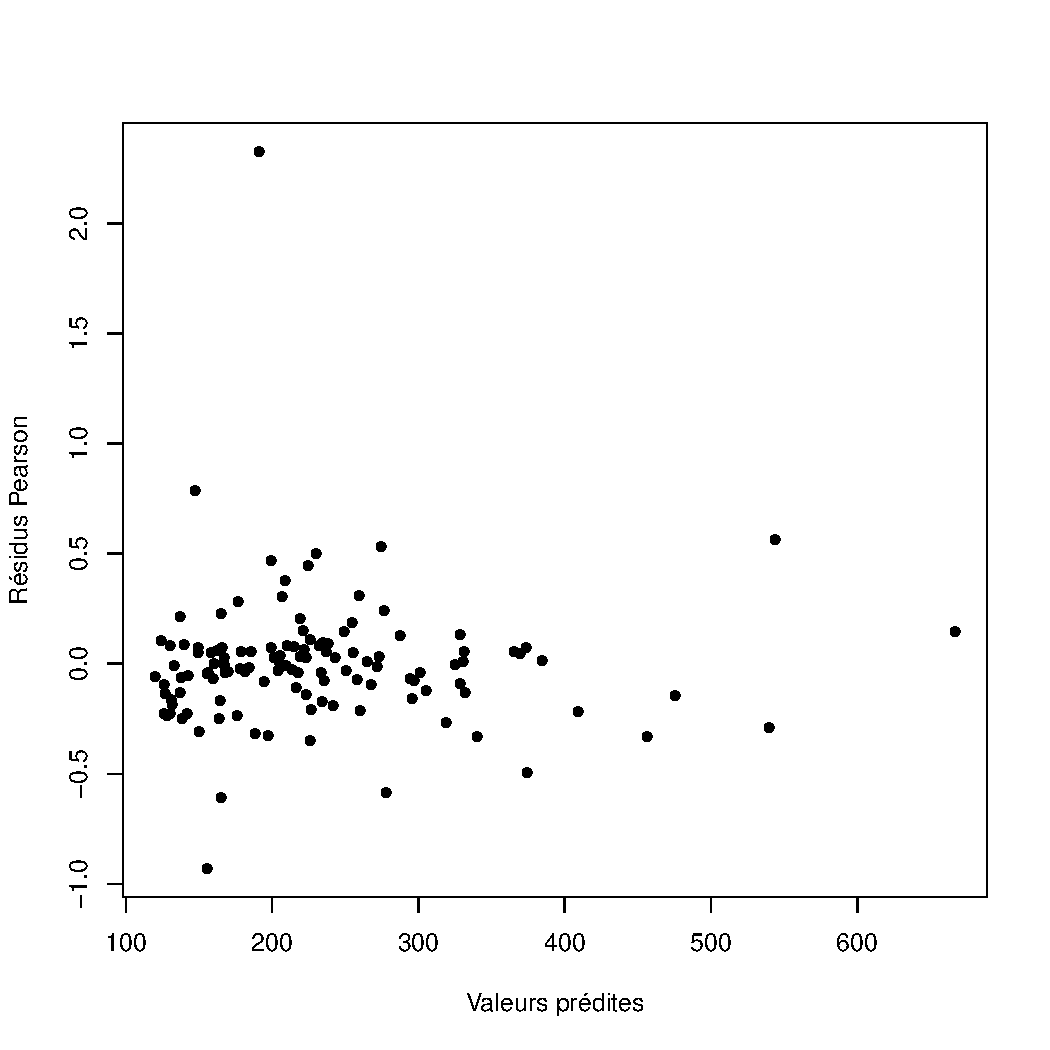
\includegraphics[width=3cm,height=3cm]{figure/unnamed-chunk-7-1}

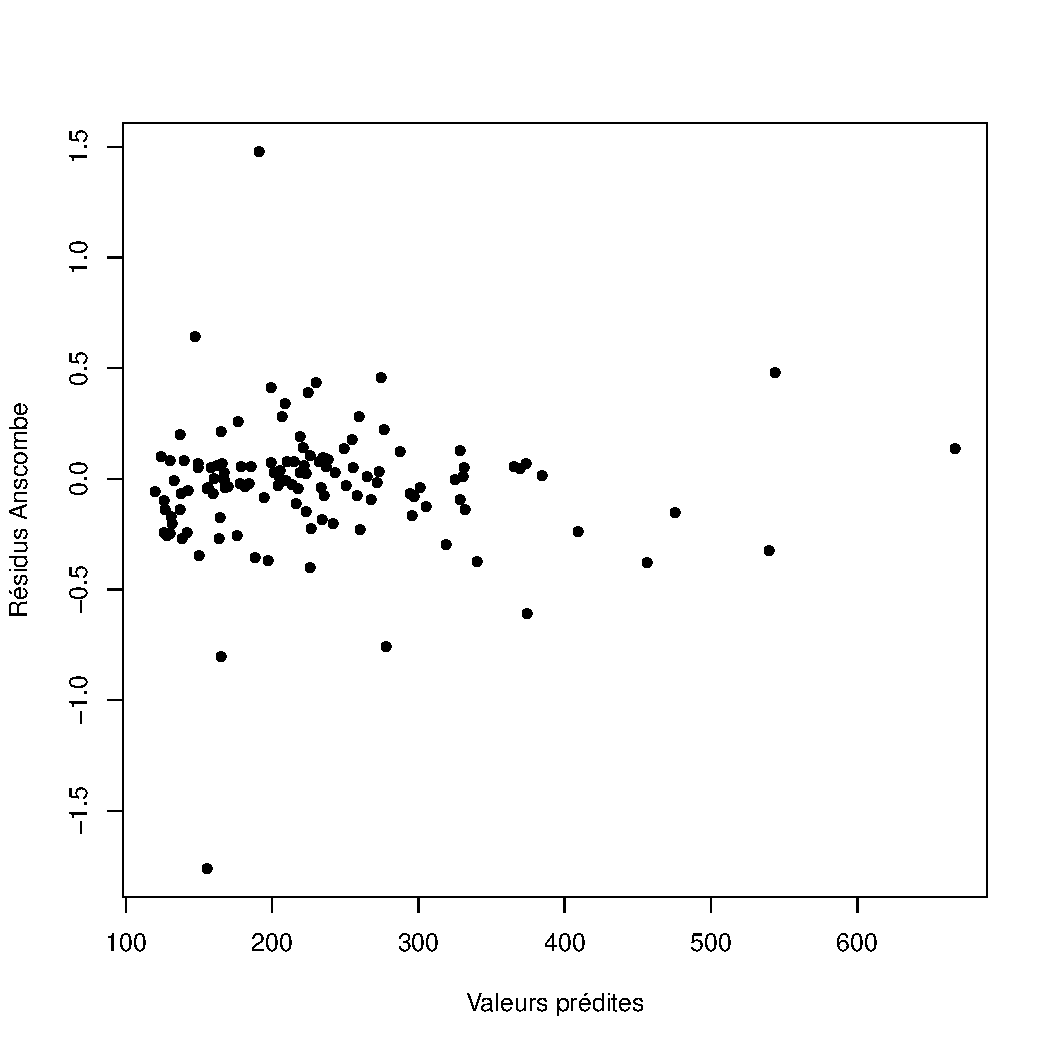
\includegraphics[width=3cm,height=3cm]{figure/unnamed-chunk-7-2}

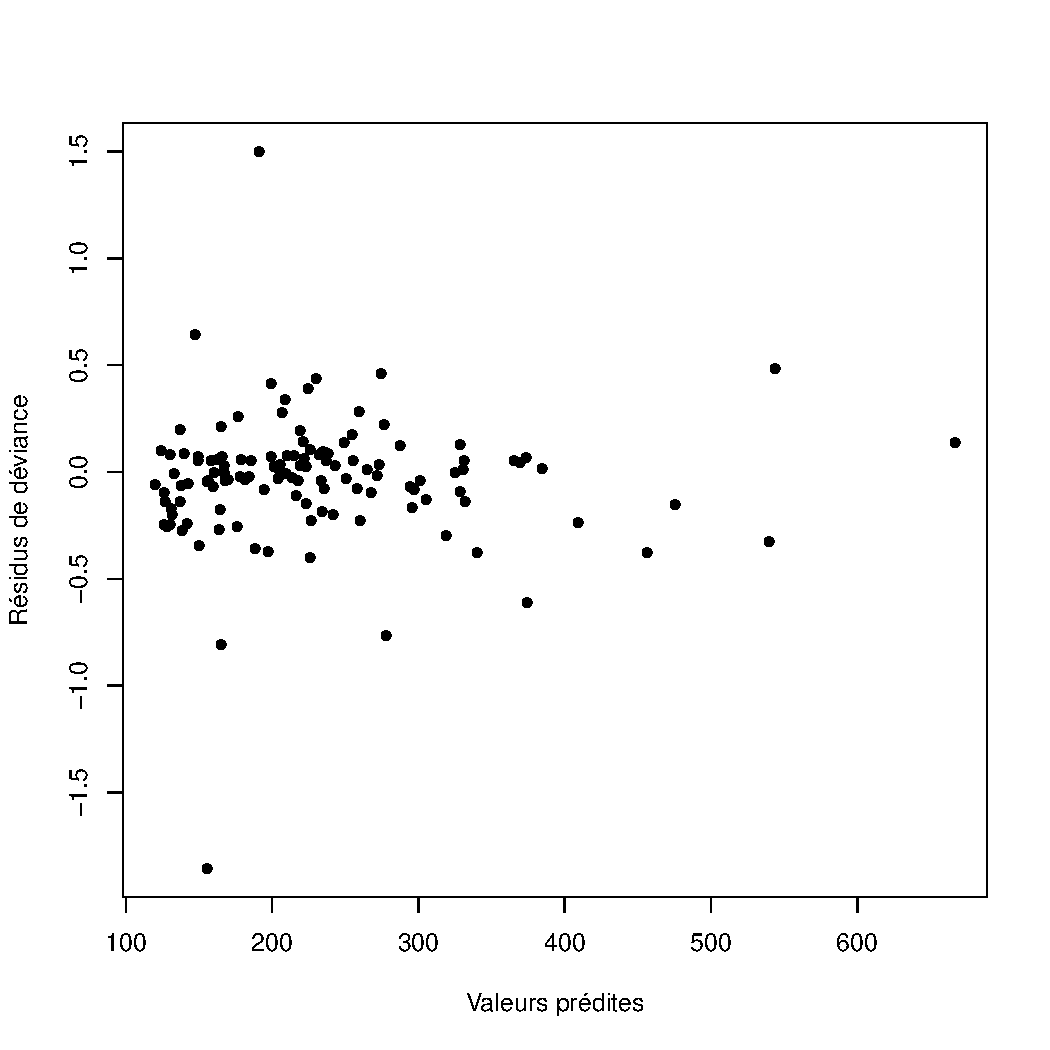
\includegraphics[width=3cm,height=3cm]{figure/unnamed-chunk-7-3}

\end{knitrout}
\caption{Résidus pour GLM Gamma}\label{fig:glm:residuals}
\end{center}
\end{figure}

\item a. Le modèle avec le lien logarithmique est

\begin{knitrout}
\definecolor{shadecolor}{rgb}{0.969, 0.969, 0.969}\color{fgcolor}\begin{kframe}
\begin{alltt}
\hlstd{modlog} \hlkwb{<-} \hlkwd{glm}\hlstd{(AvCost}\hlopt{~}\hlstd{OwnerAge}\hlopt{+}\hlstd{Model}\hlopt{+}\hlstd{CarAge,}\hlkwc{family}\hlstd{=}\hlkwd{Gamma}\hlstd{(}\hlkwc{link}\hlstd{=log),}\hlkwc{data}\hlstd{=Bcar)}
\hlkwd{summary}\hlstd{(modlog)}
\end{alltt}
\begin{verbatim}
##
## Call:
## glm(formula = AvCost ~ OwnerAge + Model + CarAge, family = Gamma(link = log),
##     data = Bcar)
##
## Deviance Residuals:
##      Min        1Q    Median        3Q       Max
## -1.84819  -0.12796  -0.00834   0.08552   1.20066
##
## Coefficients:
##                Estimate Std. Error t value Pr(>|t|)
## (Intercept)    5.711739   0.103835  55.008  < 2e-16
## OwnerAge21-24 -0.108159   0.114547  -0.944   0.3471
## OwnerAge25-29  0.005223   0.113170   0.046   0.9633
## OwnerAge30-34 -0.288090   0.113170  -2.546   0.0123
## OwnerAge35-39 -0.331420   0.114547  -2.893   0.0046
## OwnerAge40-49 -0.280775   0.113170  -2.481   0.0146
## OwnerAge50-59 -0.238136   0.113170  -2.104   0.0377
## OwnerAge60+   -0.283521   0.113170  -2.505   0.0137
## ModelB         0.057951   0.075447   0.768   0.4441
## ModelC         0.154588   0.076115   2.031   0.0447
## ModelD         0.472290   0.078497   6.017 2.43e-08
## CarAge10+     -0.735513   0.078497  -9.370 1.17e-15
## CarAge4-7     -0.111412   0.075447  -1.477   0.1426
## CarAge8-9     -0.422538   0.076115  -5.551 2.02e-07
##
## (Intercept)   ***
## OwnerAge21-24
## OwnerAge25-29
## OwnerAge30-34 *
## OwnerAge35-39 **
## OwnerAge40-49 *
## OwnerAge50-59 *
## OwnerAge60+   *
## ModelB
## ModelC        *
## ModelD        ***
## CarAge10+     ***
## CarAge4-7
## CarAge8-9     ***
## ---
## Signif. codes:
## 0 '***' 0.001 '**' 0.01 '*' 0.05 '.' 0.1 ' ' 1
##
## (Dispersion parameter for Gamma family taken to be 0.0910768)
##
##     Null deviance: 27.841  on 122  degrees of freedom
## Residual deviance: 11.263  on 109  degrees of freedom
##   (5 observations deleted due to missingness)
## AIC: 1398
##
## Number of Fisher Scoring iterations: 7
\end{verbatim}
\end{kframe}
\end{knitrout}

b. Avec ce modèle $E[Y_i]=e^{\eta_i}.$ Puisque les variables explicatives prennent toutes leur niveau de base, on a que $\hat{\eta}_i=\hat{\beta}_0=5.711739$ et $$\widehat{E[Y_i]}=e^5.711739=302.39.$$ Cela ne diffère pas beaucoup du résultat trouvé en b).

c-d-e. Puisqu'on a utilisé un lien logarithmique, on a un modèle multiplicatif. Si $e^\beta>1$, alors l'espérance du coût augmente, alors que si $e^\beta<1$ alors l'espérance du coût diminue. On peut donc tirer des conclusions similaires à celles en c), d) et e).

f. Pour un détenteur de police entre 17 et 20 ans, avec un véhicule de type D âgé de un à 3 ans, on trouve que $$\widehat{E[Y_i]}=\exp{\hat{\beta}_0+\hat{\beta}^{MODEL}_D}=\exp{5.711739+0.472290}=484.94.$$ On note que cette valeur est beaucoup moins élevée que celle obtenue en f).

g. Pour un détenteur de police entre 35 et 39 ans, avec un véhicule de type A âgé de plus de 10 ans, on trouve que $$\widehat{E[Y_i]}=\exp{\hat{\beta}_0+\hat{\beta}^{OWNERAGE}_{35-39}+\hat{\beta}^{CARAGE}_{10+}}=\exp{5.711739-0.331420-0.735513}=104.04.$$

h. La déviance $D(y,\hat{\mu})=11.263$ est donnée dans la sortie \texttt{R} pour la sous-question a). On a que $$\frac{D(y,\hat{\mu})}{\hat{\phi}}=\frac{11.263}{0.0910768}=123.66,$$ ce qui est moins près de $n-p'=109$ que pour le modèle avec le lien inverse. Le modèle semble donc moins adéquat.
\end{enumerate}
\end{solution}
\begin{solution}{2.9}
\begin{enumerate}
\item If $x_{i}$ is treated as a factor predictor with 11 levels, the linear predictor is written as $$\eta_{i}=\beta_{0}+\beta_{i} \mbox{,  } i=1,...,11$$ and $\beta_{1}=0$. The binomial density is the following: $$f_{Y}(y_{i})=\begin{pmatrix} m_{i} \\ y_{i} \end{pmatrix}\pi_{i}^{y_{i}}(1-\pi_{i})^{m_{i}-y_{i}},$$ which can be rewritten in a exponential family representation as: $$f_{Y}(y_{i})=\exp\left[y_{i}\ln\left(\frac{\pi_{i}}{1-\pi_{i}}\right)+m\ln(1-\pi_{i})+\ln\begin{pmatrix} m_{i} \\ y_{i} \end{pmatrix}\right].$$ Hence, the canonical parameter is $\theta_{i}=\ln\left(\frac{\pi_{i}}{1-\pi_{i}}\right)$ and the canonical link is the logit link. Thus,
\begin{align*}
\eta_{i}&=\ln\left(\frac{\pi_{i}}{1-\pi_{i}}\right)=\beta_{0}+\beta_{i} \\
\pi_{i}&=\frac{e^{\eta_{i}}}{1+e^{\eta_{i}}}= \frac{e^{\beta_{0}+\beta_{i}}}{1+e^{\beta_{0}+\beta_{i}}}\\
\end{align*}
The expression of the density in the reparametrization is then
\begin{align*}
f_{Y}(y_{i})&=\begin{pmatrix} m_{i} \\ y_{i} \end{pmatrix}\left(\frac{e^{\beta_{0}+\beta_{i}}}{1+e^{\beta_{0}+\beta_{i}}}\right)^{y_{i}}\left(\frac{1}{1+e^{\beta_{0}+\beta_{i}}}\right)^{m_{i}-y_{i}}\\
&=\begin{pmatrix} m_{i} \\ y_{i} \end{pmatrix}\frac{e^{y_{i}(\beta_{0}+\beta_{i})}}{(1+e^{\beta_{0}+\beta_{i}})^{m_{i}}}\\
\end{align*} The likelihood $L$ and the log-likelihood $l$ are shown below:
\begin{align*}
L(\beta_{0},...,\beta_{11};y_{1},...,y_{11})&=\prod_{i=1}^{11} \begin{pmatrix} m_{i} \\ y_{i} \end{pmatrix}\frac{e^{y_{i}(\beta_{0}+\beta_{i})}}{(1+e^{\beta_{0}+\beta_{i}})^{m_{i}}}\\
\ell(\beta_{0},...,\beta_{11};y_{1},...,y_{11})&=\sum_{i=1}^{11} \left[\ln\begin{pmatrix} m_{i} \\ y_{i} \end{pmatrix}+y_{i}(\beta_{0}+\beta_{i})-m_{i}\ln(1+e^{\beta_{0}+\beta_{i}})\right]\\
\end{align*} We have
\begin{align*}
\frac{\partial \ell}{\partial \beta_{0}}&=\sum_{i=1}^{11} \left[y_{i}-m_{i}\frac{e^{\beta_{0}+\beta_{i}}}{1+e^{\beta_{0}+\beta_{i}}}\right]\\
\frac{\partial \ell}{\partial \beta_{i}}&=y_{i}-m_{i}\frac{e^{\beta_{0}+\beta_{i}}}{1+e^{\beta_{0}+\beta_{i}}} \mbox{,  } i=2,...,11,\\
\end{align*} and $\beta_{1}=0$ by constraint of the model. The maximum likelihood estimators for the parameters are derived by solving the system of equations $\frac{\partial \ell}{\partial \beta_{i}}=0,$ $i=0,...,11$:
\begin{align*}
\sum_{i=1}^{11} \left[y_{i}-m_{i}\frac{e^{\hat{\beta}_{0}+\hat{\beta}_{i}}}{1+e^{\hat{\beta}_{0}+\hat{\beta}_{i}}}\right]&=0\\
y_{i}-m_{i}\frac{e^{\hat{\beta}_{0}+\hat{\beta}_{i}}}{1+e^{\hat{\beta}_{0}+\hat{\beta}_{i}}}&=0 \mbox{,  } i=2,...,11,\\
\Rightarrow \hat{\beta}_{0}+\hat{\beta}_{i}=\ln\left(\frac{y_{i}}{m_{i}-y_{i}}\right)& \mbox{,  } i=2,...,11,\\
\end{align*}  Using the first equation and replacing $\hat{\beta}_{0}+\hat{\beta}_{i}$ by $\ln\left(\frac{y_{i}}{m_{i}-y_{i}}\right)$,
\begin{align*}
&y_{1}-m_{1}\frac{e^{\hat{\beta}_{0}}}{1+e^{\hat{\beta}_{0}}}+\sum_{i=2}^{11} \left[y_{i}-m_{i}\frac{\left(\frac{y_{i}}{m_{i}-y_{i}}\right)}{1+\left(\frac{y_{i}}{m_{i}-y_{i}}\right)}\right]=0\\
&y_{1}-m_{1}\frac{e^{\hat{\beta}_{0}}}{1+e^{\hat{\beta}_{0}}}+\sum_{i=2}^{11} \left[y_{i}-m_{i}\frac{y_{i}}{m_{i}}\right]=0\\
&y_{1}-m_{1}\frac{e^{\hat{\beta}_{0}}}{1+e^{\hat{\beta}_{0}}}=0\\
&\hat{\beta}_{0}=\ln\left(\frac{y_{1}}{m_{1}-y_{1}}\right)\\
&\hat{\beta}_{i}=\ln\left(\frac{y_{i}}{m_{i}-y_{i}}\right)-\hat{\beta}_{0}=\ln\left(\frac{y_{i}/(m_{i}-y_{i})}{y_{1}/(m_{1}-y_{1})}\right)  \mbox{,  } i=2,...,11.\\
\end{align*}
The estimates of the model parameters are easily found in \texttt{R} as follows:
\begin{knitrout}
\definecolor{shadecolor}{rgb}{0.969, 0.969, 0.969}\color{fgcolor}\begin{kframe}
\begin{alltt}
\hlstd{(beta0} \hlkwb{<-} \hlkwd{log}\hlstd{(y[}\hlnum{1}\hlstd{]}\hlopt{/}\hlstd{(m[}\hlnum{1}\hlstd{]}\hlopt{-}\hlstd{y[}\hlnum{1}\hlstd{])))}
\end{alltt}
\begin{verbatim}
## [1] -2.917771
\end{verbatim}
\begin{alltt}
\hlstd{(beta} \hlkwb{<-} \hlkwd{c}\hlstd{(}\hlnum{0}\hlstd{,}\hlkwd{log}\hlstd{(y[}\hlopt{-}\hlnum{1}\hlstd{]}\hlopt{/}\hlstd{(m[}\hlopt{-}\hlnum{1}\hlstd{]}\hlopt{-}\hlstd{y[}\hlopt{-}\hlnum{1}\hlstd{]))}\hlopt{-}\hlstd{beta0))}
\end{alltt}
\begin{verbatim}
##  [1] 0.0000000 0.4122448 0.6151856 0.6740261 1.3083328
##  [6] 1.7137979 1.6184877 2.7636201 3.5239065 3.0178542
## [11] 3.2542430
\end{verbatim}
\end{kframe}
\end{knitrout}
Hence, here $$\hat{\beta}=(-2.9178, 0, 0.4122, 0.6152, 0.6740, 1.3083, 1.7138, 1.6185, 2.7636, 3.5239, 3.0179, 3.2542)^{T}.$$

As a consistency check following from the invariance property of maximum likelihood estimation, we can verify that the estimates of $\pi_{i}$ using the expit function are equal to the MLE estimates $\hat{\pi}_{i}=\frac{y_{i}}{m_{i}}$:
\begin{knitrout}
\definecolor{shadecolor}{rgb}{0.969, 0.969, 0.969}\color{fgcolor}\begin{kframe}
\begin{alltt}
\hlstd{(pi} \hlkwb{<-} \hlkwd{exp}\hlstd{(beta0}\hlopt{+}\hlstd{beta)}\hlopt{/}\hlstd{(}\hlnum{1}\hlopt{+}\hlkwd{exp}\hlstd{(beta0}\hlopt{+}\hlstd{beta)))}
\end{alltt}
\begin{verbatim}
##  [1] 0.05128205 0.07547170 0.09090909 0.09589041
##  [5] 0.16666667 0.23076923 0.21428571 0.46153846
##  [9] 0.64705882 0.52500000 0.58333333
\end{verbatim}
\begin{alltt}
\hlstd{y}\hlopt{/}\hlstd{m}
\end{alltt}
\begin{verbatim}
##  [1] 0.05128205 0.07547170 0.09090909 0.09589041
##  [5] 0.16666667 0.23076923 0.21428571 0.46153846
##  [9] 0.64705882 0.52500000 0.58333333
\end{verbatim}
\end{kframe}
\end{knitrout}

\item The Binomial GLM model with logit link and the linear predictor $\eta_{i}=\beta_{0}+\beta_{1}x_{i}$, $i=1,...,11$ is fitted to the data using \texttt{R} and the command:
\begin{knitrout}
\definecolor{shadecolor}{rgb}{0.969, 0.969, 0.969}\color{fgcolor}\begin{kframe}
\begin{alltt}
\hlkwd{glm}\hlstd{(}\hlkwd{cbind}\hlstd{(y,m}\hlopt{-}\hlstd{y)}\hlopt{~}\hlstd{x,}\hlkwc{family}\hlstd{=binomial)}
\end{alltt}
\end{kframe}
\end{knitrout}

The estimates of the parameters are $\hat{\beta}_{0}=-3.6070615$ and $\hat{\beta}_{1}=0.0009121$, with standard error $SE(\hat{\beta}_{0})=0.3533875$ and $SE(\hat{\beta}_{1})=0.0001084$.

\item The Binomial GLM model with probit link and the linear predictor $\eta_{i}=\beta_{0}+\beta_{1}x_{i}$, $i=1,...,11$ is fitted to the data using \texttt{R} and the command:
\begin{knitrout}
\definecolor{shadecolor}{rgb}{0.969, 0.969, 0.969}\color{fgcolor}\begin{kframe}
\begin{alltt}
\hlkwd{glm}\hlstd{(}\hlkwd{cbind}\hlstd{(y,m}\hlopt{-}\hlstd{y)}\hlopt{~}\hlstd{x,}\hlkwc{family}\hlstd{=}\hlkwd{binomial}\hlstd{(}\hlkwc{link}\hlstd{=probit))}
\end{alltt}
\end{kframe}
\end{knitrout}

The estimates of the parameters are $\hat{\beta}_{0}=-2.080$ and $\hat{\beta}_{1}=5.230\times10^{-4}$, with standard error $SE(\hat{\beta}_{0})=0.1852$ and $SE(\hat{\beta}_{1})=5.973\times10^{-5}$.

\item The Binomial GLM model with complementary log-log link and the linear predictor $\eta_{i}=\beta_{0}+\beta_{1}x_{i}$, $i=1,...,11$ is fitted to the data using \texttt{R} and the command:
\begin{knitrout}
\definecolor{shadecolor}{rgb}{0.969, 0.969, 0.969}\color{fgcolor}\begin{kframe}
\begin{alltt}
\hlkwd{glm}\hlstd{(}\hlkwd{cbind}\hlstd{(y,m}\hlopt{-}\hlstd{y)}\hlopt{~}\hlstd{x,}\hlkwc{family}\hlstd{=}\hlkwd{binomial}\hlstd{(}\hlkwc{link}\hlstd{=cloglog))}
\end{alltt}
\end{kframe}
\end{knitrout}

The estimates of the parameters are $\hat{\beta}_{0}=-3.360$ and $\hat{\beta}_{1}=7.480\times10^{-4}$, with standard error $SE(\hat{\beta}_{0})=0.3061$ and $SE(\hat{\beta}_{1})=8.622\times10^{-5}$.

\item Predictions can be found using the inverse of the link function. For the model with canonical link (model from b), we find that $$\hat{y}_{2000}=\frac{e^{\hat{\beta}_{0}+2000\hat{\beta}_{1}}}{1+e^{\hat{\beta}_{0}+2000\hat{\beta}_{1}}}=0.1439472.$$ Alternatively, the command \texttt{predict(modelb,data.frame(x=2000),type="response",se.fit=TRUE)} can be used to calculate the predictions and associated standard errors. The resulting predictions and standard errors are presented in Table~\ref{tab:glm:pred}. The probability of developing fissures after 2000 hours of operations is 14.39\% according to model b, and the standard deviation is 2.08\%. This prediciton is quite comparable with the complementary log-log model (d), for which the estimated probability of developing fissures is 14.36\%, with a standard error of 2.03\%. The precision is slightly better in this model than the two others due to a smaller variance. The estimated probability with Model c, using the probit link, is higher at 15.06\%, with standard error of 2.06\%.
\begin{table}[htbp]
\begin{center}
\begin{tabular}{|l||c|c|c|}
  \hline
   & Model b (logit link) & Model c (probit link) & Model d (compl. log-log link) \\
  \hline
  \hline
	 $\hat{y}_{2000}$ &0.1439472 & 0.150615 & 0.1436447\\ \hline
	 $SE(\hat{y}_{2000})$ &0.02080256 & 0.02062154 & 0.02030803 \\ \hline
\end{tabular}
\caption{Predictions and Standard Errors for Predictions for the 3 Models} \label{tab:glm:pred}
\end{center}
\end{table}

\item Figure~\ref{fig:glm:modfit} shows a plot of the data points along with the three fitted lines. It was obtained using the following code in \texttt{R}, where \texttt{ilogit, iprobit} and \texttt{icloglog} are the inverse of the corresponding link functions:
\begin{knitrout}
\definecolor{shadecolor}{rgb}{0.969, 0.969, 0.969}\color{fgcolor}\begin{kframe}
\begin{alltt}
\hlkwd{plot}\hlstd{(x,y}\hlopt{/}\hlstd{m,}\hlkwc{pch}\hlstd{=}\hlnum{19}\hlstd{,}\hlkwc{xlab}\hlstd{=}\hlstr{"Number of Hours of Operation (x)"}\hlstd{,}
     \hlkwc{ylab}\hlstd{=}\hlstr{"Prob of Developing Fissures"}\hlstd{)}
\hlstd{j} \hlkwb{<-} \hlkwd{seq}\hlstd{(}\hlnum{0}\hlstd{,}\hlnum{4800}\hlstd{,}\hlnum{1}\hlstd{)}
\hlkwd{lines}\hlstd{(j,}\hlkwd{ilogit}\hlstd{(}\hlkwd{coef}\hlstd{(modelb)[}\hlnum{1}\hlstd{]}\hlopt{+}\hlkwd{coef}\hlstd{(modelb)[}\hlnum{2}\hlstd{]}\hlopt{*}\hlstd{j),}\hlkwc{lwd}\hlstd{=}\hlnum{2}\hlstd{)}
\hlkwd{lines}\hlstd{(j,}\hlkwd{iprobit}\hlstd{(}\hlkwd{coef}\hlstd{(modelc)[}\hlnum{1}\hlstd{]}\hlopt{+}\hlkwd{coef}\hlstd{(modelc)[}\hlnum{2}\hlstd{]}\hlopt{*}\hlstd{j),}\hlkwc{lty}\hlstd{=}\hlnum{2}\hlstd{,}\hlkwc{col}\hlstd{=}\hlnum{2}\hlstd{,}\hlkwc{lwd}\hlstd{=}\hlnum{2}\hlstd{)}
\hlkwd{lines}\hlstd{(j,}\hlkwd{icloglog}\hlstd{(}\hlkwd{coef}\hlstd{(modeld)[}\hlnum{1}\hlstd{]}\hlopt{+}\hlkwd{coef}\hlstd{(modeld)[}\hlnum{2}\hlstd{]}\hlopt{*}\hlstd{j),}\hlkwc{lty}\hlstd{=}\hlnum{3}\hlstd{,}\hlkwc{col}\hlstd{=}\hlnum{4}\hlstd{,}\hlkwc{lwd}\hlstd{=}\hlnum{2}\hlstd{)}
\hlkwd{legend}\hlstd{(}\hlstr{"topleft"}\hlstd{,}\hlkwc{legend}\hlstd{=}\hlkwd{c}\hlstd{(}\hlstr{"Logit"}\hlstd{,}\hlstr{"Probit"}\hlstd{,}\hlstr{"Complementary log-log"}\hlstd{),}
       \hlkwc{lty}\hlstd{=}\hlkwd{c}\hlstd{(}\hlnum{1}\hlstd{,}\hlnum{2}\hlstd{,}\hlnum{3}\hlstd{),}\hlkwc{col}\hlstd{=}\hlkwd{c}\hlstd{(}\hlnum{1}\hlstd{,}\hlnum{2}\hlstd{,}\hlnum{4}\hlstd{),}\hlkwc{lwd}\hlstd{=}\hlkwd{rep}\hlstd{(}\hlnum{2}\hlstd{,}\hlnum{3}\hlstd{))}
\end{alltt}
\end{kframe}
\end{knitrout}


\begin{figure}[htbp]
\begin{center}
\begin{knitrout}
\definecolor{shadecolor}{rgb}{0.969, 0.969, 0.969}\color{fgcolor}
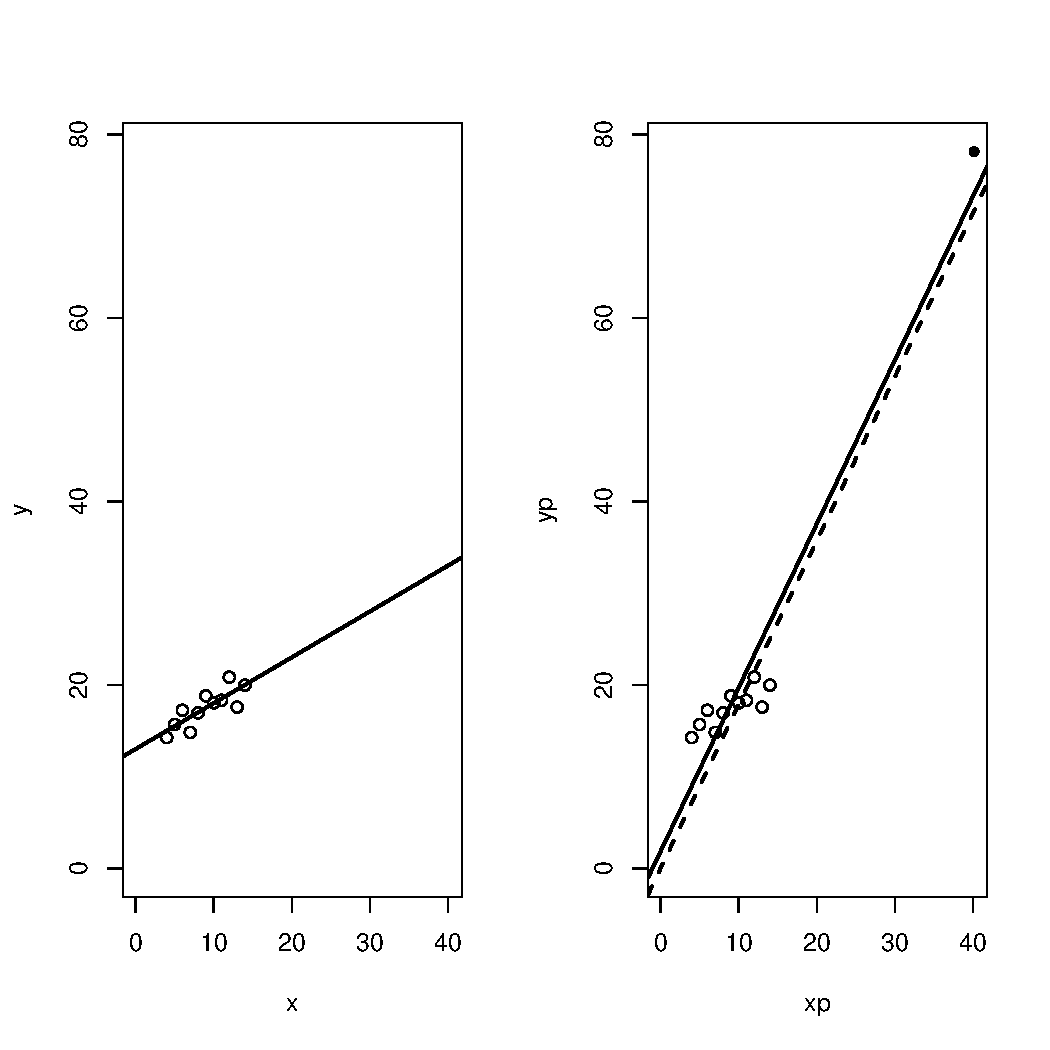
\includegraphics[width=\maxwidth]{figure/unnamed-chunk-17-1}

\end{knitrout}
\end{center}
\caption{Logistic, Probit and Complementary Log-Log Model Fit} \label{fig:glm:modfit}
\end{figure}

It is easy to observe that the fit is better when the number of hours of operations is lower, it seems that the variance of the observations is increasing with the predictor. This is expected in a generalized linear model framework. The three fitted lines are slightly different. The probit link produces lower estimates in the tails and higher estimates in the middle of the range of the predictors. It seems like this model is less representative of the data than the others. The complementary log-log model (d) predicts higher probabilities of failures in the extremes of the range of the predictors. This seems to fit the data well, and recall that the variance of the predictions where also smaller than other models in this case, which is a desirable property. The line for the model with canonical link is between the two others. It could also be a reasonable model for the data.

\end{enumerate}
\end{solution}
